\documentclass{5220hw}
\usepackage{amsmath,amssymb,latexsym, mathtools}
\usepackage{verbatim}
\usepackage{algorithm}
\usepackage{listings}
\usepackage{courier}
\usepackage{algpseudocode}
\usepackage{changepage}

\lstset{basicstyle=\ttfamily,breaklines=true}

\begin{document}

\name{Sheroze Sheriffdeen}
\netid{mss385}

\maketitle

\begin{exercises}

\item The class cluster consists of eight nodes and fifteen Xeon Phi accelerator boards.  Based on an online search for information on these systems, what do you think is the theoretical peak flop rate (double-precision floating point operations per second)?  Show how you computed this, and give URLs for where you got the parameters in your calculation.  (We will return to this question again after we cover some computer architecture.) \\

According to the Intel calculations, the theoretical peak flop rate for a single Xeon Phi 5110p coprocessor is,
16 FLOPS/clock x 60 cores x 1.053 GHz = 1010.88 GF/s. 
\footnote{https://www-ssl.intel.com/content/www/us/en/benchmarks/server/xeon-phi/xeon-phi-theoretical-maximums.html} 

16 FLOPS/clock comes from a 512-bit wide Vector Processing Unit. That is 8 double precision FMA operations which amounts to 16 double precision instructions per clock cycle. 
\footnote{http://www.training.prace-ri.eu/uploads/tx\_pracetmo/MIC\_Intro\_Architecture.pdf}

According to the Intel spec,\footnote{http://download.intel.com/support/processors/xeon/sb/xeon\_E5-2600.pdf} the peak flop rate for the Intel Xeon E5-2620 v3 processors is 120GF/s. 

We have 15 Xeon Phis and $8 * 12$ Intel Xeon E5-2620 v3 processors leading to a, \\
$1010.88 * 15 + 96 * 120 = 26.68$ TF/s of total theoretical peak flop rate. \\

\item What is the approximate theoretical peak flop rate for your own machine? \\

I have a Mid 2014 Retina MacBook Pro. It has a Intel Core i5-4278U processor with a base frequency of 2.6 GHz and two cores. The flop rate is then 2 * 2.6 = 5.2 GF/s. \\

\item Suppose there are $t$ tasks that can be executed in a pipeline with $p$ stages.  What is the speedup over serial execution of the same tasks? \\

Let $u$ be the time per stage. Assume that all stages take the same amount of time. \\
Then, the time for the serial execution is $tu$. \\
With a pipeline, the time taken is $pu + (t-1)u$. \\
The speedup is then, $\dfrac{t}{p + t -1}$. \\

\item Consider the following list of tasks (assume they can't be pipelined): \\

compile GCC (1 hr) \\
compile OpenMPI (0.5 hr) - depends on GCC \\
compile OpenBLAS (0.25 hr) - depends on GCC \\
compile LAPACK (0.5 hr) - depends on GCC and OpenBLAS \\
compile application (0.5 hr) - depends on GCC, OpenMPI, OpenBLAS, LAPACK \\

What is the minimum serial time between starting to compile and having a compiled application? \\
GCC + OpenMPI + OpenBLAS, LAPACK + Application : 2.75 hours. \\ 
What is the minimum parallel time given an arbitrary number of processors? \\
GCC + (OpenMPI and OpenBLAS in parallel) + (LAPACK after OpenBLAS parallel with OpenMPI) + Application: 2.25 hours. \\

\item Clone the membench repository from GitHub:
\begin{lstlisting}
git clone git@github.com:cornell-cs5220-f15/membench.git
\end{lstlisting}

On your own machine, build `membench` and generate the associated plots; for many of you, this should be as simple as typing `make` at the terminal (though I assume you have Python with pandas and Matplotlib installed; see also the note about Clang and OpenMP in the leading comments of the Makefile).  Look at the output file timings-heat.pdf; what can you tell about the cache architecture on your machine from the plot? \\

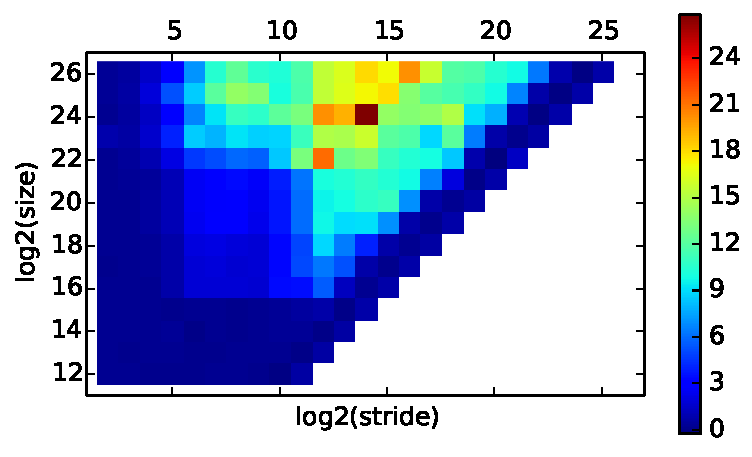
\includegraphics[scale=0.9]{membench/timings-heat.pdf} \\
The worst performant region is when the stride is $2^{14}$ and the size is $2^{24}$. 
\item From the cloned repository, check out the totient branch:

\begin{lstlisting}
git checkout totient
\end{lstlisting}

You may need to move generated files out of the way to do this. If you prefer, you can also look at the files on GitHub. Either way, repeat the exercise of problem 5.  What can you tell about the cache architecture of the totient nodes? \\

\includegraphics[scale=0.9]{membench/timings-heat_totient.pdf} \\

\item Implement the following three methods of computing the centroid of a million two-dimensional coordinates (double precision). Time and determine which is faster:

\begin{enumerate}
    \item  Store an array of (x,y) coordinates; loop i and simultaneously sum the xi and yi. \\
		Time taken: 3.882146e-02 (1.03036 GFLop/s)


    \item Store an array of (x,y) coordinates; loop i and sum the xi, then sum the yi in a separate loop \\
		Time taken: 5.588314e-02 (0.715779 GFLop/s)
		
    \item Store the xi in one array, the yi in a second array. Sum the xi, then sum the yi. \\
    		Time taken: 2.763550e-02 (1.44741 GFLop/s) (Fastest)
\end{enumerate}



\end{exercises}

\end{document}
